\chapter{Methods}
\label{ch:methods}
\section{The scikit-learn library}It was chosen to implement algorithms from the scikit-learn module of the python language since it "exposes a wide variety of machine learning algorithms, both supervised and unsupervised, using a consistent, task-oriented interface, thus enabling easy comparison of methods for a given application" \cite{Pedregosa2012}. This allowed several different algorithms to be implemented within the same environment and gain meaningful results with minimal prior coding and analysis. The algorithms initially chosen was decision trees (DT's) since these allow both regression and classification analysis, and are known as 'white boxes' due to their relatively transparent process whereby the mechanics of training could be evaluated more readily. 

\section{Decision Trees}
Different machine learning algorithms use different statistical procedures in order to evaluate data and make inferences. DT's emulate a logical classification procedure similar to that used in biology to identify species. Starting from the full dataset a series of binary if-then tests are consequentially performed and data split into 2 branches continuously until a final statistical criterion is satisfied. The algorithm does this by arbitrarily choosing a value that splits the parameter space in 2, forming a node and 2 branches. A statistical test (purity measure), either Gini impurity or entropy of information gain, is then applied to the 2 child datasets separately to evaluate how correlated the members within each child are, and the resulting values summed proportionately to find the total purity. Decision trees then recurse through the parameter space in a greedy fashion to find those that maximise the purity, and selects this for the split. Once found, the process repeats on each of the child datasets until a predefined stopping criterion is fulfilled, producing a leaf at the end of each branch. This results in a series of rules that can be applied to unseen data in an attempt to reproduce the classifications.\
The Gini impurity is defined as:
\begin{equation}
H(X_m) = \sum_k p_{mk} (1 - p_{mk}),
\end{equation}
and the entropy defined as:
\begin{equation}
H(X_m) = -\sum_k p_{mk} \log{ p_{mk}, 
\end{equation}
where the target classification takes on value $0,1,..,k-1$ for node $m$, representing a region $R_{m}$ with $N_{m}$ observations. For a single input variable $x_{i}$ with class label $y_{i}$ (i.e. fast/slow rotation), the proportion of class $k$ observations in node $m$ is given by:
\begin{equation}
p_{mk} = 1/N_{m} \sum_{x_{i}\subset{R_{m}}} I(y_{i}=k)
\end{equation}
In the case of entropy, the purity is measured in terms of entropy gain, defined as the entropy of the parent minus the entropy of the child.\\
The benefits of decision trees are that they are more interpretable, employing a 'white box' approach, compared to other algorithms (i.e. neural nets) that have a relatively opaque process. They require little data preparation compared to others that need, for example normalisation, and are well suited to binary decision classes as well as being fast.
The backend of the SKlearn modules were not evaluated directly and implemented na\"{i}vely. The parameters were initialised to their defaults as described in the documentation\cite{sklearn}. Using the modules themselves required elementary use of python to pass the module arrays of necessary values. Implementation proceeded in 2 stages once the data had been suitably formatted. The data was arbitrarily split into 2 groups, a training and a test set, based solely on their position within the results: they were ordered according to their LEDA classification and occupied different locations of the sky, and so should not have any bias. For classification, the training set was passed to the module as a list with each item holding the feature value (i.e. S\'{e}rsic index) or a list of feature values if more than one feature used, and target variable (i.e. fast/slow rotator classification, spin parameter value). A function was output that incorporated the learned rules which was then applied to the test data set resulting in an array of predicted values that could be measured against the known values.\
The algorithm was run as a classification problem due to the more simple analysis of success and errors. This is because it allowed the success to be evaluated in a more elementary fashion, without recourse to analysing more complex error distributions.
Decision tree and random forest methods were then applied and the parameters adjusted manually to achieve optimal results. The parameters evaluated are outlined in the following section.
\subsection{Parameters}
SKLearn allows several parameters to be adjusted manually in order to maximise the efficiency of the models, and these are particular to each. For decision trees, these are outlined in the attached table.
\begin{table}[H]
\caption {SKLearn Decision Tree Parameters} \label{tab:dectreeparams}
\renewcommand{\arraystretch}{1.0} % this reduces the vertical spacing between rows
\linespread{1.0}\selectfont\centering
\begin{tabu} to \textwidth { | c | l | p{7cm} | }
	\hline
	Parameter & Options & Description \\
	\hline
	Criterion  & Gini or Entropy  & Uses the gini impurity as outlined above or entropy for information gain. The gini impurity default was used \\
	\hline
	Splitter & Best  or Random & Chooses the best split or the best random split to make at each node based on the criterion. \\
	\hline
	max\textunderscore features & int & Considers the maximum number of features of the dataset to consider when recursing for the best split. \\
	\hline
	max\textunderscore depth & int or None & The maximum depth of the tree, i.e. how many splits the tree makes. The default of None will recurse until all leaves are pure, i.e. contain 1 class, or contain less than the min\textunderscore samples\textunderscore split.\\
	\hline
	min\textunderscore samples\textunderscore split & int,float (default=2) & The minimum number of samples required to be at a leaf node, where the leaf node represents the split into classifications.\\
	\hline
	max\textunderscore leaf\textunderscore nodes & int, none (default=None) & The maximum number of leaf nodes allowed, with the tree choosing nodes which best minimises the gini impurity.\\
	\hline
	min\textunderscore weight\textunderscore fraction\textunderscore leaf & float or None & The minimum weighted fraction of the sum total of weights (of all the input samples) required to be at a leaf node. Samples have equal weight when sample\textunderscore weight is not provided. No weights were supplied since and so were equally weighted.\\ %COULD USE THIS BASED ON ERRORS??\\
	\hline
	min\textunderscore impurity\textunderscore split & float (default=1e-7) & Threshold for early stopping in tree growth. A node will split if its impurity is above the threshold, otherwise it splitting will cease and the node forms a leaf.\\
	\hline
	presort & bool, (default=False) & Option to possibly speed up training process, not used here.\\
	\hline
\end{tabu}
\end{table}

\section{Data \& Formatting}
\subsection{ATLAS\textsuperscript{3D}}
Spectroscopic data (namely S\'ersic index of the single fit and bulge component, n and $n_{b}$ respectively,  and D/T, the Disk-to-Total light ratio) was extracted from \cite{Krajnovic2013} whilst the kinematic parameters $\lambda_{Re}$, $\lambda_{Re/2}$ and the Fast/Slow rotation classification were extracted from \cite{Emsellem2011}. The data from both sources was combined using a pandas dataframe.\\
The classifier was first trained using the spin parameter $\lambda_{Re}$ with the FS rotation classification as target variable as a test measure, which successfully predicted 100\% of the test set. The data was then evaluated for statistical correlations between spectroscopic parameters and the spin parameter. This was performed using the inbuilt scatter matrix command of the pandas module that plots each variable against the other, with the diagonal used to depict the kernel density estimation (kde) which estimates the probability density function of the variable. This was performed for the full dataset and for the two rotator populations individually.\\As can be seen from the figures, there are no immediately obvious distinguishing features that separate the two populations. The $R_{max}$ population peaks at around 0.8 with a much sharper peak for FR's compared to a broader distribution centred at 0.6 for SR's. The ellipticity for FR's exhibits a double peak at 0.2 and 0.6, values ranging from 0.0-0.9 while SR's exhibit a single peak centred at 0.2 but a smaller range of 0.0-0.5. The D/T ratios share very similar distributions but FR's have flatter maximums and minimums. The Se\'rsic index distributions are almost identical for both populations with a peak at n=2 and an extended tail towards higher values, except that SR's have a significant number of galaxies with n=1, indicating a tendency to have a purely exponential profile, whilst the Se\'rsic index of the bulge had a larger range of 0-11 compared to 0-9, but with a similar lineshape with peak at $n_{b}\approx$0.2 compared to peak at $n_{b}\approx$0.6. The flattening of the bulge component, $q_{b}$, had minimum and maximum at 0.25 and 0.75 respectively, but for the fast rotators there was a second smaller peak at 0.0. Both populations exhibited 2 peaks at 0.0 and 18.0 for the effective surface brightness, although the second peak at the higher value was more pronounced for SR's. The flattening of the exponential component $q_{d}$ distributions were very similar in both cases, centred at 0.0, except for a shallower tail skewed to higher values in FR's. Both populations also had a peak centred at $\approx$21. \\
These plots indicate that there are few if any distinct distinguishing features by which the rotation classification can be categorically determined. The fact, however, that there are multiple variables that do vary slightly between the populations suggests that a machine learning algorithm could identify some empirical rules combining these traits to achieve such an aim.

\begin{sidewaysfigure}[ht]
	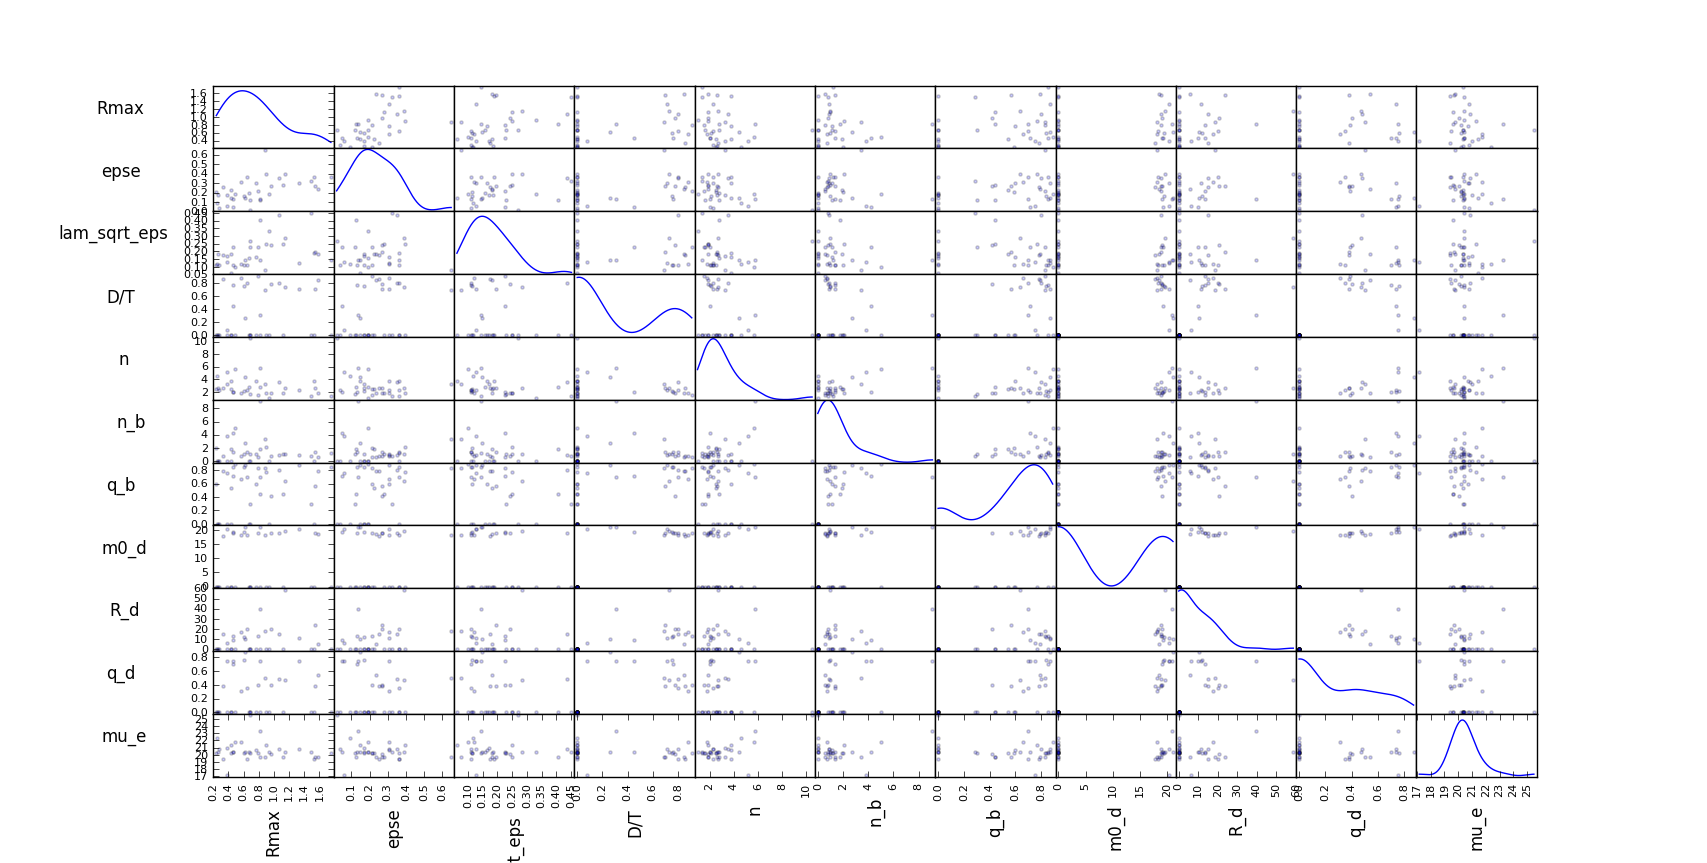
\includegraphics[width=\textwidth,height=\textheight,keepaspectratio]{scatter_matrix_slow_rots_rotlabels}
	\caption{Scatter matrix of the slow rotator population}
	\label{fig:MatSlow}
\end{sidewaysfigure}

\begin{sidewaysfigure}[ht]
	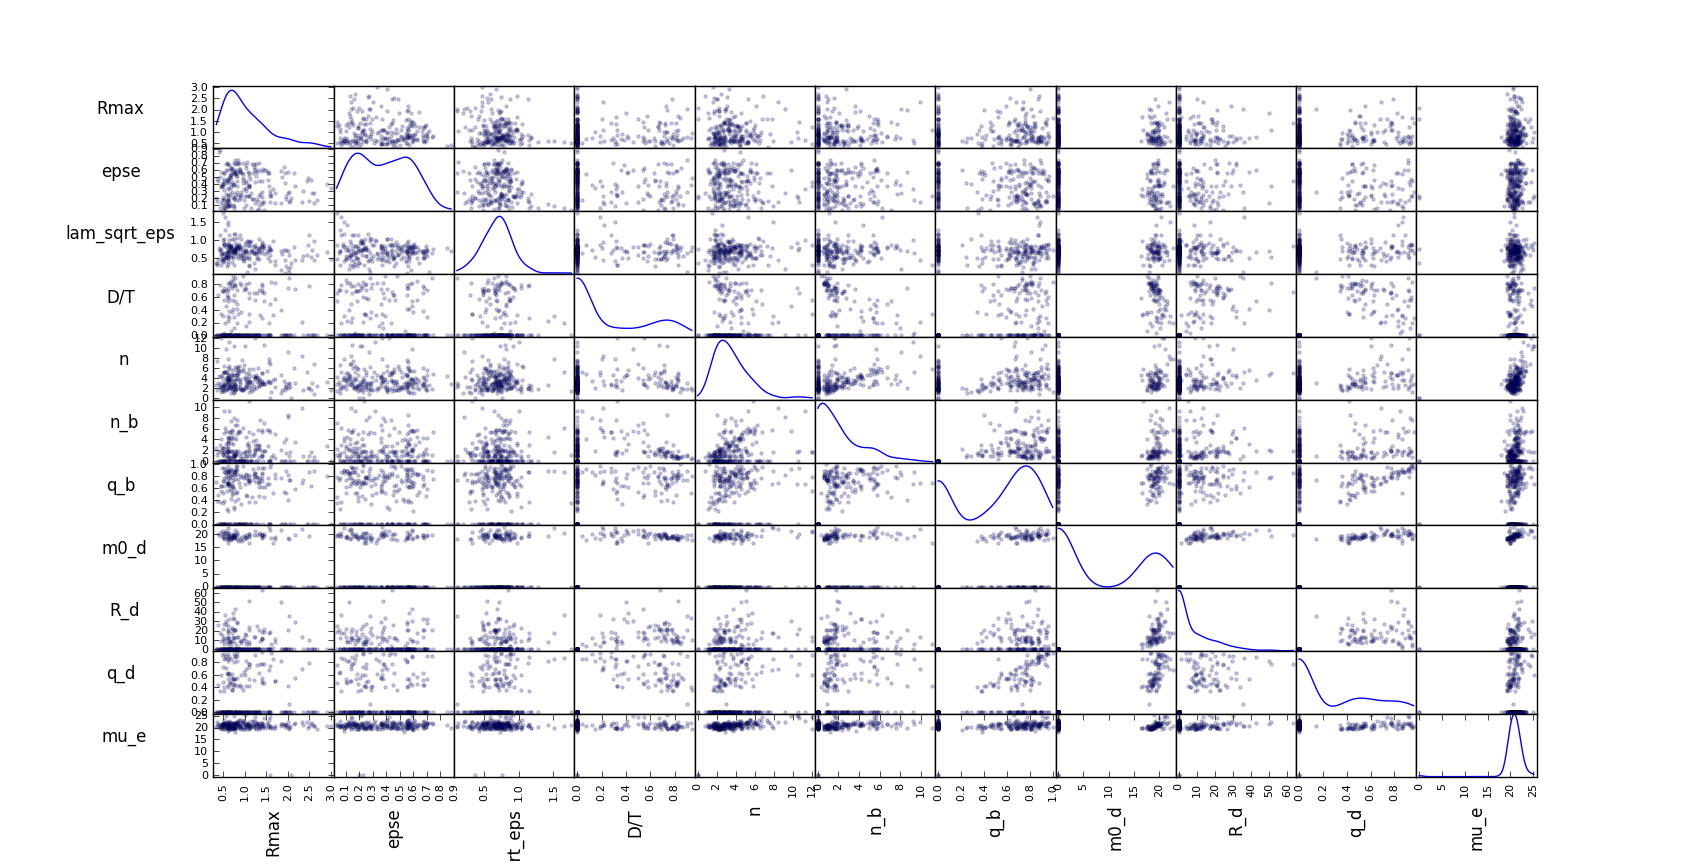
\includegraphics[width=\textwidth,height=\textheight,keepaspectratio]{scatter_matrix_fast_rots_rotlabels}
	\caption{Scatter matrix of the fast rotator population}
	\label{fig:MatFast}
\end{sidewaysfigure}
